\subsection{MOSFET Threshold Voltage}

We first wish to find properties of the MOSFET, these results are found in Table \ref{tab:VBB0}.

By varying $V_{GS}$ we can estimate $V_T$ which is found to be: 1.58V

\begin{table}[h]
    \begin{tabular}{@{}ccccc@{}}
\toprule
\textbf{$V_{BB}$ (V)} & \multicolumn{1}{l}{\textbf{$V_{GG}$ (V)}} & \textbf{$V_{DD}$ (V)} & \textbf{$V_{DS}$ (V)} & \textbf{$I_{DS}$} \\ \midrule
%                        VGG     VDD     VDS     IDS
\textit{\textbf{0}}     &  2.86     &   7.09    &  6.0550     & 1.0108      \\
\textit{\textbf{0}}     &  3.60     &   8.15    &  6.0768       &  2.0041     \\
\textit{\textbf{0}}     &  4.22     &   9.13    &  6.0277     & 3.0031      \\
\textit{\textbf{0}}     &  4.76     &   10.17    & 6.0273      & 4.0049      \\
\textit{\textbf{0}}     &  5.27     &   11.21    & 6.0167       &   5.0176    \\ \bottomrule
\end{tabular}
    \caption{MOSFET characteristics at $V_{BB}$ = 0}
    \label{tab:VBB0}
\end{table}

For each of $V_{BB}$ = -2, -6, -10 we repeat the measurements, and these are shown in Tables below:

\begin{table}[ht]
    \begin{tabular}{@{}ccccc@{}}
\toprule
\textbf{$V_{BB}$ (V)} & \multicolumn{1}{l}{\textbf{$V_{GG}$ (V)}} & \textbf{$V_{DD}$ (V)} & \textbf{$V_{DS}$ (V)} & \textbf{$I_{DS}$} \\ \midrule
%                        VGG     VDD     VDS     IDS
\textit{\textbf{-2}}     &  4.48     &  7.06     & 6.0200       &  1.0062     \\
\textit{\textbf{-2}}     &  5.18     &  8.07     & 6.0013      &  2.0049     \\
\textit{\textbf{-2}}     &  5.75     &  9.12     & 3.0004      & 6.0210      \\
\textit{\textbf{-2}}     &  6.27     &  10.21     & 4.0233      &  6.0476     \\
\textit{\textbf{-2}}     &  6.75     &  11.20     & 5.0190      &  6.0050     \\ \bottomrule
\end{tabular}
    \caption{MOSFET characteristics at $V_{BB}$ = -2}
    \label{tab:VBB2}
\end{table}

\begin{table}[ht]
    \begin{tabular}{@{}ccccc@{}}
\toprule
\textbf{$V_{BB}$ (V)} & \multicolumn{1}{l}{\textbf{$V_{GG}$ (V)}} & \textbf{$V_{DD}$ (V)} & \textbf{$V_{DS}$ (V)} & \textbf{$I_{DS}$} \\ \midrule
%                        VGG     VDD     VDS     IDS
\textit{\textbf{-6}}     &  6.64     & 7.05      & 6.0200      &1.0014       \\
\textit{\textbf{-6}}     &  7.31     & 8.12      & 6.0434       & 2.0131      \\
\textit{\textbf{-6}}     &  7.86     & 9.12      & 6.0099      & 3.0064      \\
\textit{\textbf{-6}}     &  8.36     & 10.19      & 6.0380       & 4.0219       \\
\textit{\textbf{-6}}     &  8.81     & 11.22      & 6.0200      & 5.0171      \\ \bottomrule
\end{tabular}
    \caption{MOSFET characteristics at $V_{BB}$ = -6}
    \label{tab:VBB6}
\end{table}

\begin{table}[ht]
    \begin{tabular}{@{}ccccc@{}}
\toprule
\textbf{$V_{BB}$ (V)} & \multicolumn{1}{l}{\textbf{$V_{GG}$ (V)}} & \textbf{$V_{DD}$ (V)} & \textbf{$V_{DS}$ (V)} & \textbf{$I_{DS}$} \\ \midrule
%                        VGG     VDD     VDS     IDS
\textit{\textbf{-10}}     & 8.28      & 7.05      & 6.0195      & 1.0019      \\
\textit{\textbf{-10}}     & 8.93      & 8.14      & 6.0714      & 2.0046      \\
\textit{\textbf{-10}}     & 9.48      & 9.16      & 6.0354       & 3.0200      \\
\textit{\textbf{-10}}     & 9.96      & 10.19      & 6.0191      & 4.0268      \\
\textit{\textbf{-10}}     & 10.41      &  11.21     &  6.0154     & 5.0133      \\ \bottomrule
\end{tabular}
    \caption{MOSFET characteristics at $V_{BB}$ = -10}
    \label{tab:VBB10}
\end{table}

\subsection{Semiconductor Parameter Analyzer}

See included for various data curves which are used to describe the MOSFET device.

\begin{figure}[ht]
    \centering
    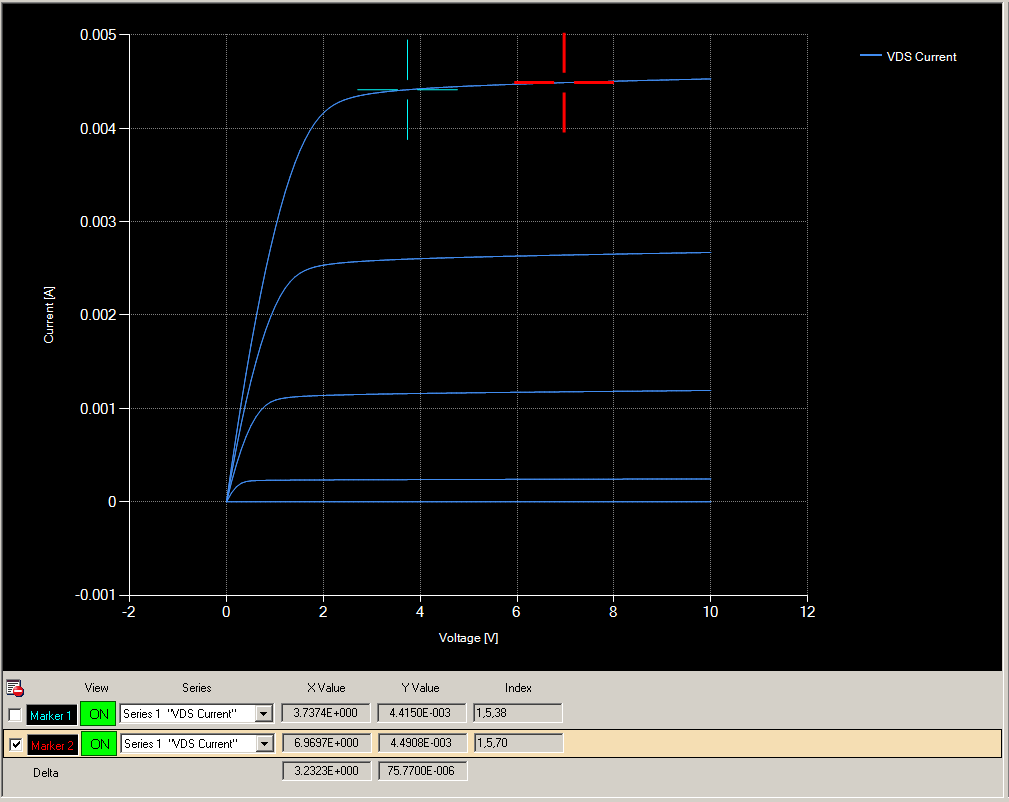
\includegraphics[width=.95\linewidth]{figures/Graph_For_Output_Resitance.PNG}
    \caption{Drain-to-Source current vs Gate-to-Source voltage. The markers compare the highest $V_{GS}$ to constant $V_{GS}$ and are used to find the output resistance.}
    \label{fig:VGS_varied}
\end{figure}

\begin{figure}[ht]
    \centering
    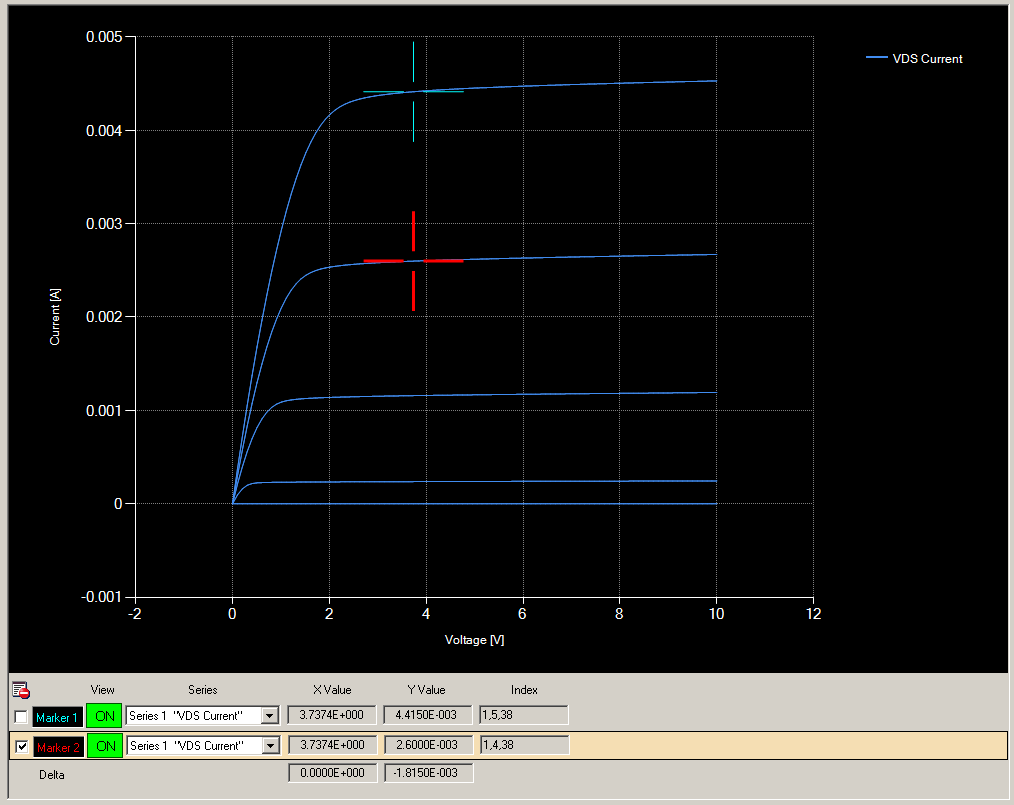
\includegraphics[width=.95\linewidth]{figures/Graph_For_Output_TransCon.PNG}
    \caption{Drain-to-Source current vs Gate-to-Source voltage. The markers are used to find $g_m$, the MOSFET transconductance at saturation}
    \label{fig:VGS_constant}
\end{figure}